There exist two types of basic modules in \posl: \oms{} and \opchs{}. A \om{} is a function receiving an input, then executes an internal algorithm, and returns an output. A \opch{} is also a function receiving and returning information, but in contrast, the \opch{} can receive information from two different ways: through parameter or from outside, i.e. by communicating with a module from another solver.

\subsection{Computation Module}

%In this sub-section we expose the definition and the characteristics and the details of the \om, and give some examples. We explain how to create new \oms{} using the basic layer of the framework.

A \om{} is the most basic and abstract way to define a piece of computation. It is a function receiving an input, then executing an internal algorithm, and returning an output. The input and output types will characterize the computation module signature. It can be dy\-na\-mi\-cally replaced by or combined with other computation modules, since they can be shared among solvers working in parallel. They are joined through \ass.

\defname{Computation Module}{
A \om{} $Cm$ is a mapping defined by: 
\begin{equation}
\label{def:om}
Cm:D \rightarrow I
\end{equation}
}

$D$ and $I$ can be either a set of configurations, or set of sets of configurations, or a set of values of some data type, etc.

Consider a local search meta-heuristic solver. One of its \oms{} can be the function returning the set of configurations composing the neighborhood of a given configuration:

\begin{equation*}
Cm_{neighborhood}:D_1\times D_2\times\dots\times D_n \rightarrow 2^{D_1\times D_2\times\dots\times D_n}
\end{equation*}

\noindent where $D_i$ represents the definition domains of each variable of the input confi\-gura\-tion.

Figure~\ref{fig:om} shows an example of computation module: it receives a configuration $S$ and then computes the set $V$ of its neighbor configurations $\left\{S^1, S^2, \dots, S^m\right\}$.

\vspace{0.5cm}
\begin{figure}
	\centering	
	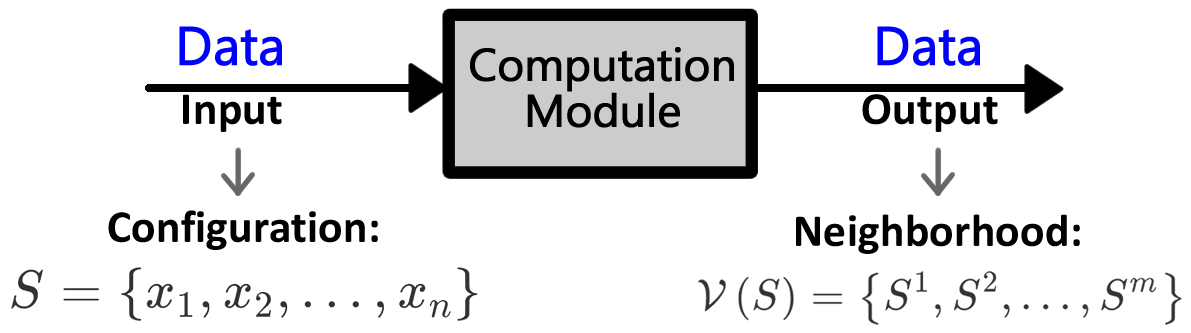
\includegraphics[width=0.7\linewidth]{OM.png}
	\caption{An example of a computation module computing a neighborhood}\label{fig:om}
\end{figure}

\subsection{Communication modules}

%In this sub-section we expose the definition and the characteristics and the details of the \opch, and give some examples. We explain how to create new \opchs{} using the basic layer of the framework.

A \opch{} is also a function receiving and returning its information, but in contrast, the \opch{} can receive information from two different ways: through input or from outside, i.e., by communicating with a module from another solver. A \opch{} is the component in charge of the information reception in the communication between solvers (we will talk about information transmission in the next section). They can interact with \oms{} through operators (see Figure~\ref{fig:och}).

A \opch{} can receive two types of information, always coming from an external solver: data or \oms{}. It is important to notice that when we are talking about sending/receiving \oms, we mean sending/receiving only required information to identify it and being able to instantiate it.

In order to distinguish from the two types of \opchs, we will call Data Communication Module the \opch{} responsible for the data reception (Figure~\ref{subfig:doch}), and Object Communication Module the one responsible for the reception and instantiation of \oms{} (Figure~\ref{subfig:ooch}).

\defname{Data Communication Module}{
A \emph{Data Communication Module} $Ch$ is a component that produces a mapping defined as follows: 
\begin{equation}
\label{def:dopench}
Ch:U \rightarrow I
\end{equation}
It returns the information $I$ coming from an external solver, no matter what the input $U$ is.
}

\defname{Object Communication Module}{
	If we denote by $\mathbb{M}$ the space of all the \oms{} defined by Definition \ref{def:om}, then an \emph{Object Communication Module} $Ch$ is a component that produces a \om{} coming from an external solver as follows:
	\begin{equation}
	\label{def:oopench}
	Ch:\mathbb{M} \rightarrow \mathbb{M}
	\end{equation}
}%

\begin{figure}
	\centering
	\subfloat[][Data \opch]{
		\label{subfig:doch}
		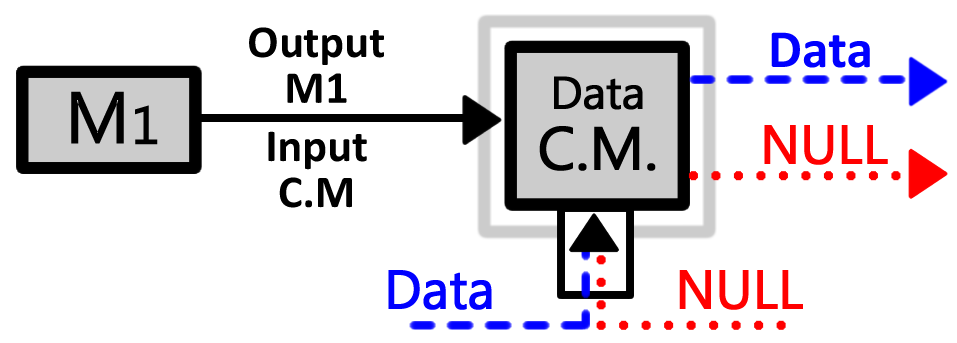
\includegraphics[width=0.4\linewidth]{D_OCh.png}
	}
	\hspace{0.05\textwidth}%
	\subfloat[][Object \opch]{%
		\label{subfig:ooch}
		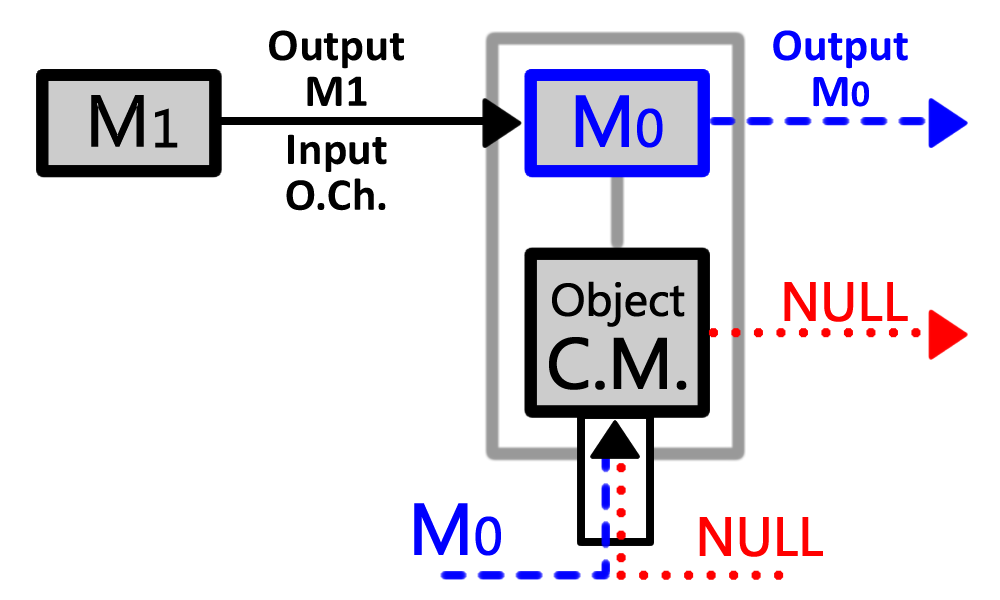
\includegraphics[width=0.4\linewidth]{O_OCh.png}
	}
	\caption[]{Communication module}
	\label{fig:och}
\end{figure}

Users can implement new computation and connection modules but \posl{} already contains many useful modules for solving a broad range of problems.

Due to the fact that \opchs{} receive information coming from outside and have no control on them, it is necessary to define the {\it NULL} information, to denote the absence of any information. If a Data Communication Module receives a piece of information, it is returned automatically. If a Object Communication Module receives a \om{}, the latter is instantiated and executed with the \opch's input, and its result is returned. In both cases, if no available information exists (no communications performed), the \opch{} returns the {\it NULL} object.